\section{Imagen}

Imagen \cite{imagen} is a text-to-image diffusion model that builds on the power of large transformer language models \cite{transformer} (LLMs) to generate high-fidelity images. The combination of diffusion (section \ref{subsec:diffusion_models}) and LLMs have shown remarkable outputs. One of the main observation in the paper that the researchers discovered is that a \textbf{large frozen LLM has bigger impact on the fidelity of generated images than increasing the amount of parameters in the image diffusion model}. Another contribution in the paper is the introduction of new benchmark called \textbf{DrawBench} to evaluate text-to-image models such as DALL-E \cite{dalle}, VQ-GAN+CLIP \cite{vqgan_clip}, latent diffusion models \cite{stable_diffusion}, GLIDE \cite{glide}, and DALLE-E 2 \cite{dalle_2}.

The researchers achieved a new state-of-the-art COCO FID score of 7.27, and human raters prefer Imagen in terms of image-text alignment with reference images. On DrawBench the researchers found Imagen outperforms state-of-the-art DALL-E 2 model in human evaluation on text-to-image task. But most importantly, the use of large pre-trained frozen language models was found to be instrumental to both image fidelity and image-text alignment.













\subsection{Text-to-Text Transfer Transformer (T5)}

\textbf{T}ext-\textbf{t}o-\textbf{T}ext \textbf{T}ransfer \textbf{T}ransformer (T5) \cite{t5_model} is a model that was introduced by Google Research that treats tasks as a text-to-text problems. For example, for summorization tasks we could prompt the LLM: "Please summorize the following: ...", for translation tasks we could prompt the LLM: "Translate from English to French the word 'You'", as well as for text classification, question answering, conversations, and other tasks. In short, this knowledge can be viewed as developing a 'general-purpose' model that can understand text.  Instead of explicitly training the model to learn words or text, such as in the case of \textbf{word vectors} \cite{cbow_word2vec}, a more common practice is to \textbf{pre-train} \cite{bert} the model on data-rich task in an unsupervised manner. The model T5 is open-source and was trained on large corpura of textual data. The base version of the model (T5-base) consists of 220 million parameters, while the largest version of the model (T5-XXL) consists of 11 billion parameters. In the context of Imagen, the Imagen model uses a frozen version of T5-XXL model to encode conditional text prompts.

This pre-training approach causes the model to develop general-purpose abilities that are then used in downstream tasks (translation, summorization, conversation and more). Unsupervised pre-training is appealing because unlabeled text data is abundant and available on the Internet. For example, the Common Crawl project \cite{common_crawl_project} is a non-profit organization that crawls the internet and provides free access to its achived datasets to the publlic. A lot of research has been done on the training of models on large scale dataset, and the consensus is that the larger the dataset, the better the model performs \cite{radford2019language} \cite{jozefowicz2016exploring} \cite{hestness2017deep}. The T5 models were trained on the "Colossal Clean Crawled Corpus" (C4) dataset, which consists of 750GB of English text data scraped from the web.

The architecture of T5 consists of an encoder-decoder transformer model, closly follows the implementation in the paper that introduced the transformer model \cite{transformer}. It first maps an input token sequence to embeddings, which are passed to the encoder. The encoder consists of stacked blocks, each with a \textbf{self-attention layer} (section \ref{subsec:cross_attention}) followed by a feed-forward network (simple fully connected layer). Layer normalization (appendix \ref{appendix:layer_normalization}) is applied before each component, using a simplified version without additive bias \footnote{Layer normalization rescales and shifts the activations of a layer by rescaling values (e.g. between 0 and 1) and by additive bias. Removing the additive bias means the model won't apply the extra shift; it only rescales the activations without any other adjustments.}. Residual connections and dropout are applied throughout. The decoder mirrors the encoder but includes an additional attention layer to attend to encoder outputs and uses autoregressive self-attention to focus on past outputs. The final decoder output passes through a dense layer with shared weights from the input embeddings. 

\textbf{The training objective} of T5 model is called \textbf{span corruption}, which is stronger version of \textbf{masked language modeling}. Given a sentence, some words and some contigous words are masked (in masked language modeling, only single words are masked), and the model should predict those words. For example: "Thank you for inviting me to your party last week", where the masked words are "for inviting" and "last". And the model should predict those words in the following sentence: "Thank you [MASKED] me to your party [MASKED] week". The model should learn to reconstruct the missing text. The actual loss function is to choose the correct words by similarity in the embeddings space, which is where cross-entropy is commonly used for.

\begin{figure}[h]
    \centering
    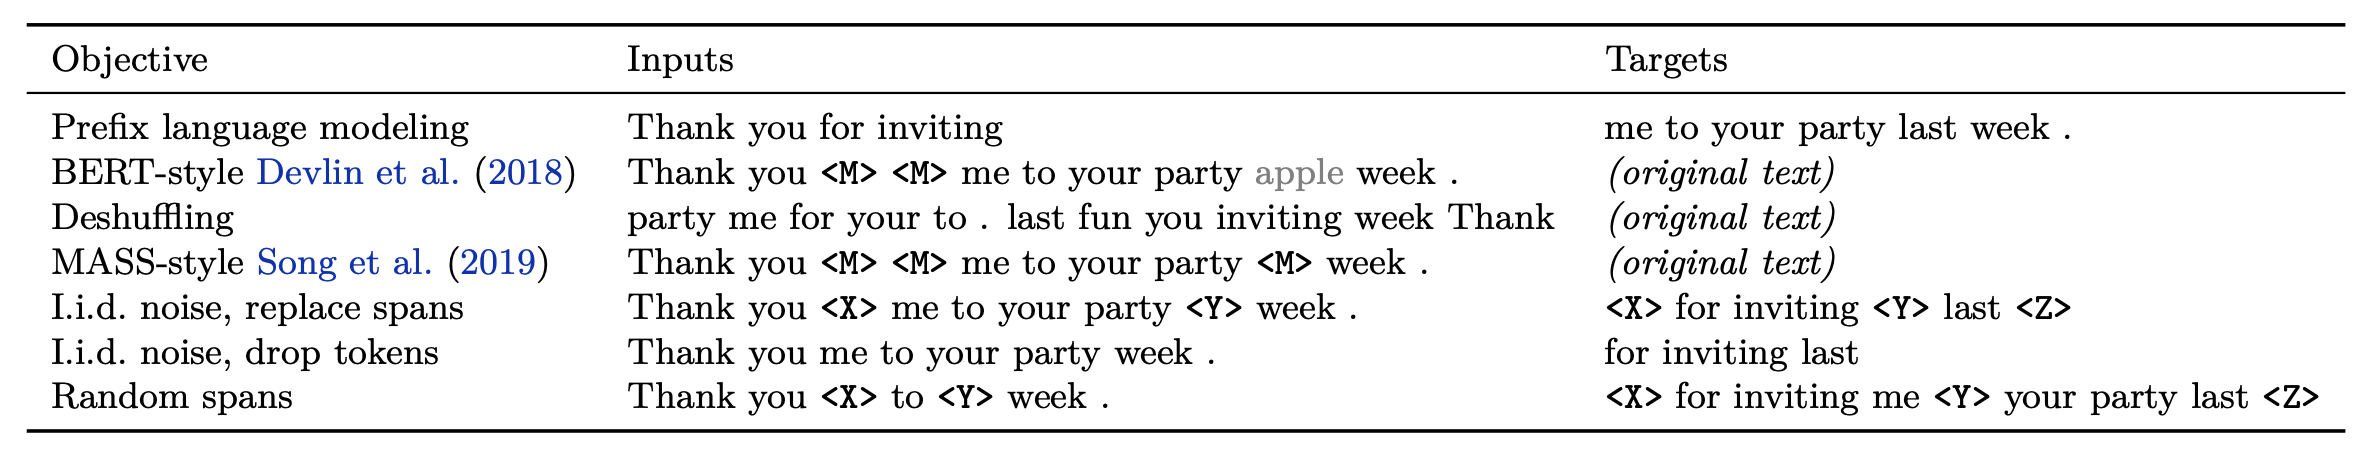
\includegraphics[width=1\textwidth]{images/imagen/t5_objectives.png}
    \caption{The unsupervised training objectives of T5 model. \textless M\textgreater\ denotes shared mask token (the same mask token is used to represent all masked positions in the input). \textless X\textgreater, \textless Y\textgreater, and \textless Z\textgreater\ denote sentiel tokens (with unique token IDs, they mark specific masked positions that the model should reconstruct).}
\end{figure}














\subsection{Pretrained text encoders}

In the paper, the researchers explored some of the biggest and most advanced text encoders: \textbf{T5-XXL} \cite{t5_model}, \textbf{GPT} \cite{gpt} \cite{mingpt} \cite{gpt_another}, and \textbf{BERT} \cite{bert}. These large language models (LLMs) are trained exclusively on text datasets, which are substantially larger compared to image-text pair datasets (as used in models like CLIP). Additionally, these models serve as significantly larger text encoders than those designed to handle image-text pairs alone.

Freezing these models \footnote{When we freeze models we generally mean that some (or all) of the parameters of the model are not changed during training. How? When a layer is frozen during training, no gradient updates will occur for this layer. Gradients will still flow from frozen layer to non-frozen layer, it doesn't skip the backpropogation. It just passes the gradients from the next layer to the previous layer.} (pre-training) provides significant advantage over training them: less memory and computation consumption during training (of the text-to-image model). They also found that scaling the text encoder size improves the quality of the generated images.














\subsection{Diffusion guidance weight}

As described before (section \ref{subsec:classifier_free_diffusion_guidance}), there are two methods to increase sample quality with the tradeoff of diversity:

\begin{itemize}
    \item \textbf{Classifier guidance} uses a separate, pre-trained classifier model to guide the image generation process in diffusion models by adjusting the noise based on how closely the generated image matches a desired condition.
    
    \item \textbf{Classifier-free guidance} (CFG) removes the need for a separate classifier by training the diffusion model itself to optionally condition on the label or text input, enabling the model to guide the generation internally, improving efficiency and reducing computational complexity.
\end{itemize}

More formally, in CFG, sampling is performed weighting the conditional and unconditional signals:

\begin{equation}
    \underbrace{\tilde{\epsilon}_\theta (z_t, c)}_{\text{adj noise prediction}} = \underbrace{w \epsilon_\theta (z_t, c)}_{\text{conditional score}} + \underbrace{(1 - w) \epsilon_\theta (z_t)}_{\text{unconditional score}}
    \label{eq:classifier_free_guidance}
\end{equation}

where $\epsilon_\theta$ is the noise prediction with the learned parameters $\theta$, $w$ is the \textbf{guidance weight} (conditional weight), $c$ is the condition, and $z_t$ is the latent variable at timestep $t$.

The researchers conducted experiments and found that increasing the guidance weight improves image-text alignment but reduces image fidelity, producing unnatural images. Its caused by \textbf{train-test mismatch}: looking at equation \ref{eq:classifier_free_guidance} if we set $w$ to 1, then the model won't be trained on unconditional samples. This causes the model to generate outputs that exceed the noise prediction (in the paper they refer to this as "x-prediction") in the normalized range of [-1, 1]. And when iteratively applying the model to its own outputs at each step, errors caused by this mismatch accumulate, which causes unnatural outputs.

For this reason they investigated static thresholding and dynamic thresholding.

\textbf{Static thresholding} is a method of applying the clipping operation to force the x-prediction output to fit to the normalized range of [-1, 1]. However, static thresholding still result in over-saturated and less detailed images as the guidance weight approaches 1.

% TODO: I dont really understand dynamic thresholding, need to read more about it.
\textbf{Dynamic thresholding} is a new method developed by the researchers. Instead of clipping the x-prediction to the normalized range, dynamic thresholding sets a threshold $s$ based on the distribution of absolute pixel values in the current x-prediction, allowing the threshold to adapt to the specific output of the model at that moment. In other words, if the pixel values are saturated (close to the [-1, 1] range), dynamic thresholding pushes them inwards by thresholding in the range [-$s$, $s$] and then dividing by $s$.

\begin{figure}
    \centering
    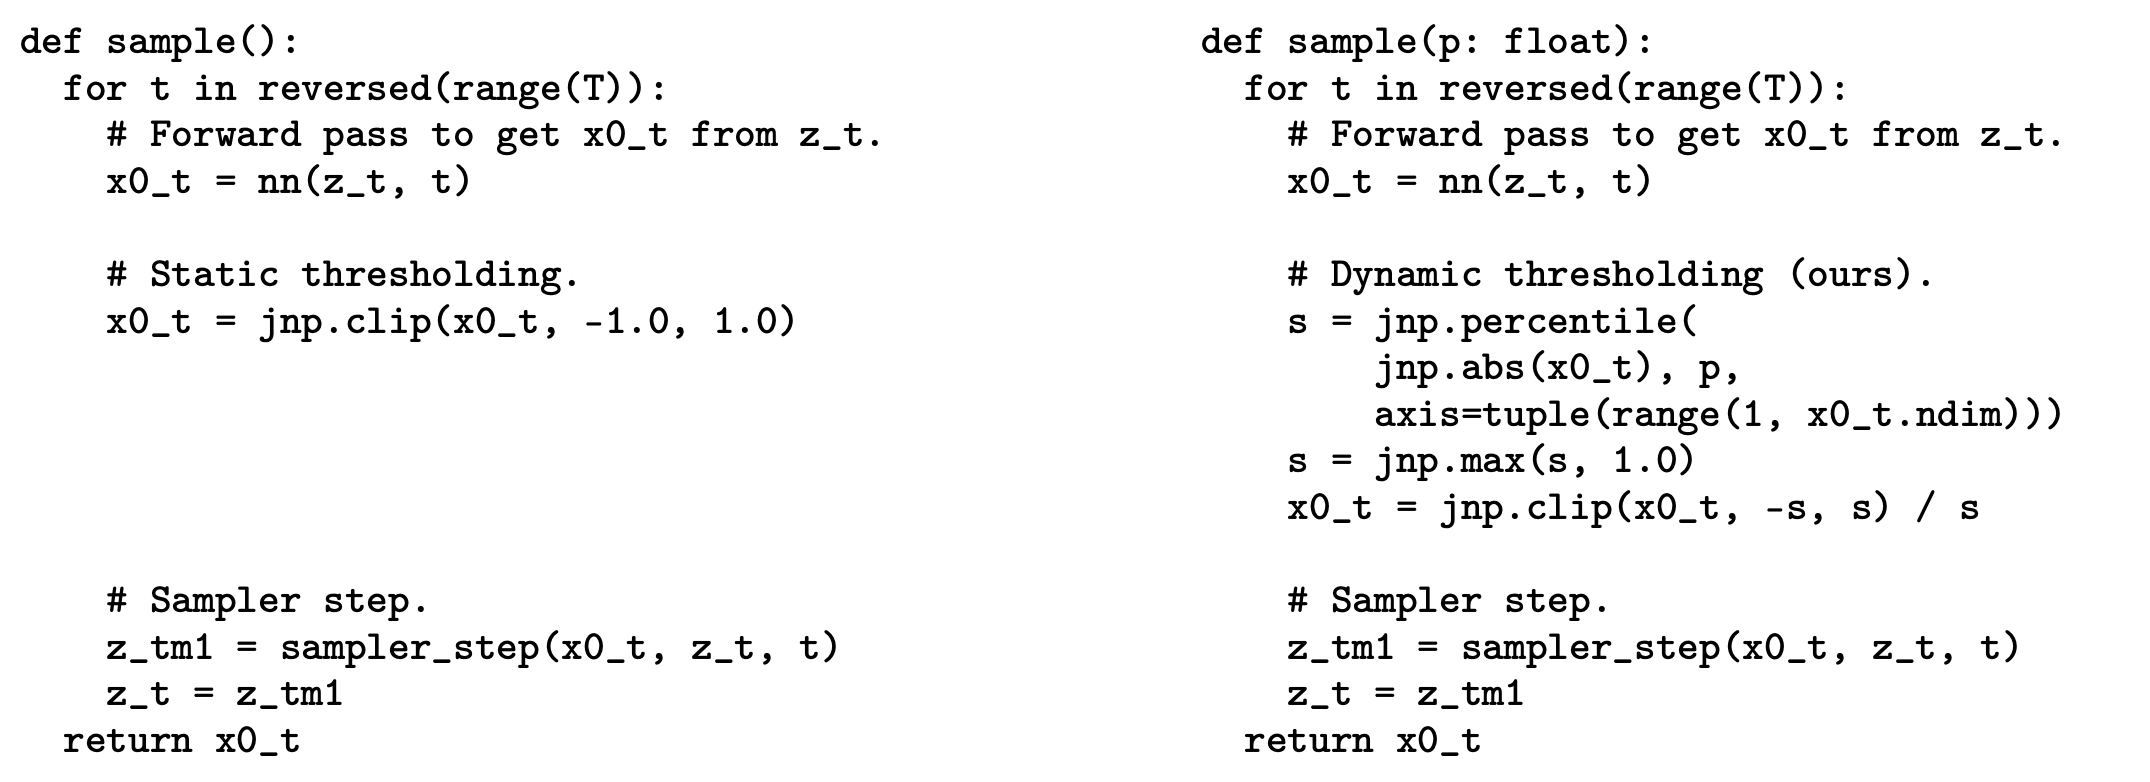
\includegraphics[width=0.75\textwidth]{images/imagen/static_dynamic_thresholding.png}
    \caption{Static (left) and dynamic (right) thresholding code implementation.}
    \label{fig:dynamic_thresholding}
\end{figure}

The implementation of static and dynamic thresholding is shown in figure \ref{fig:dynamic_thresholding}.











\subsection{Architecture}

An overview of Imagen architecture is shown in figure \ref{fig:imagen_architecture}.

It consists of a T5-XXL (T5-Extra Extra Large) text encoder, which maps text prompts (as conditioning signal) to embeddings. The T5-XXL model has 11 billion parameters, and its the largest version of the T5 model.

Then these embeddings are then fed into a 64x64 image diffusion model (the output image resolution is 64x64). These 64x64 images are then fed to a 256x256 super-resolution diffusion model (that increases the resolution from 64x64 to 256x256). And finally, a final 1024x1024 super-resolution diffusion model is used to again increase the resolution of the final image. All the diffusion models are conditioned on the same text embeddings.

"\textbf{Cascaded diffusion models}" is the term for chaining multiple super-resolution (diffusion) models together. The state-of-the-art GLIDE \cite{glide} model also uses cascaded diffusion models.

Similar to Stable Diffusion (LDMs), Imagen also uses classifier-free guidance \cite{classifier_free_guidance} (section \ref{subsec:classifier_free_diffusion_guidance}).

\begin{figure}
    \centering
    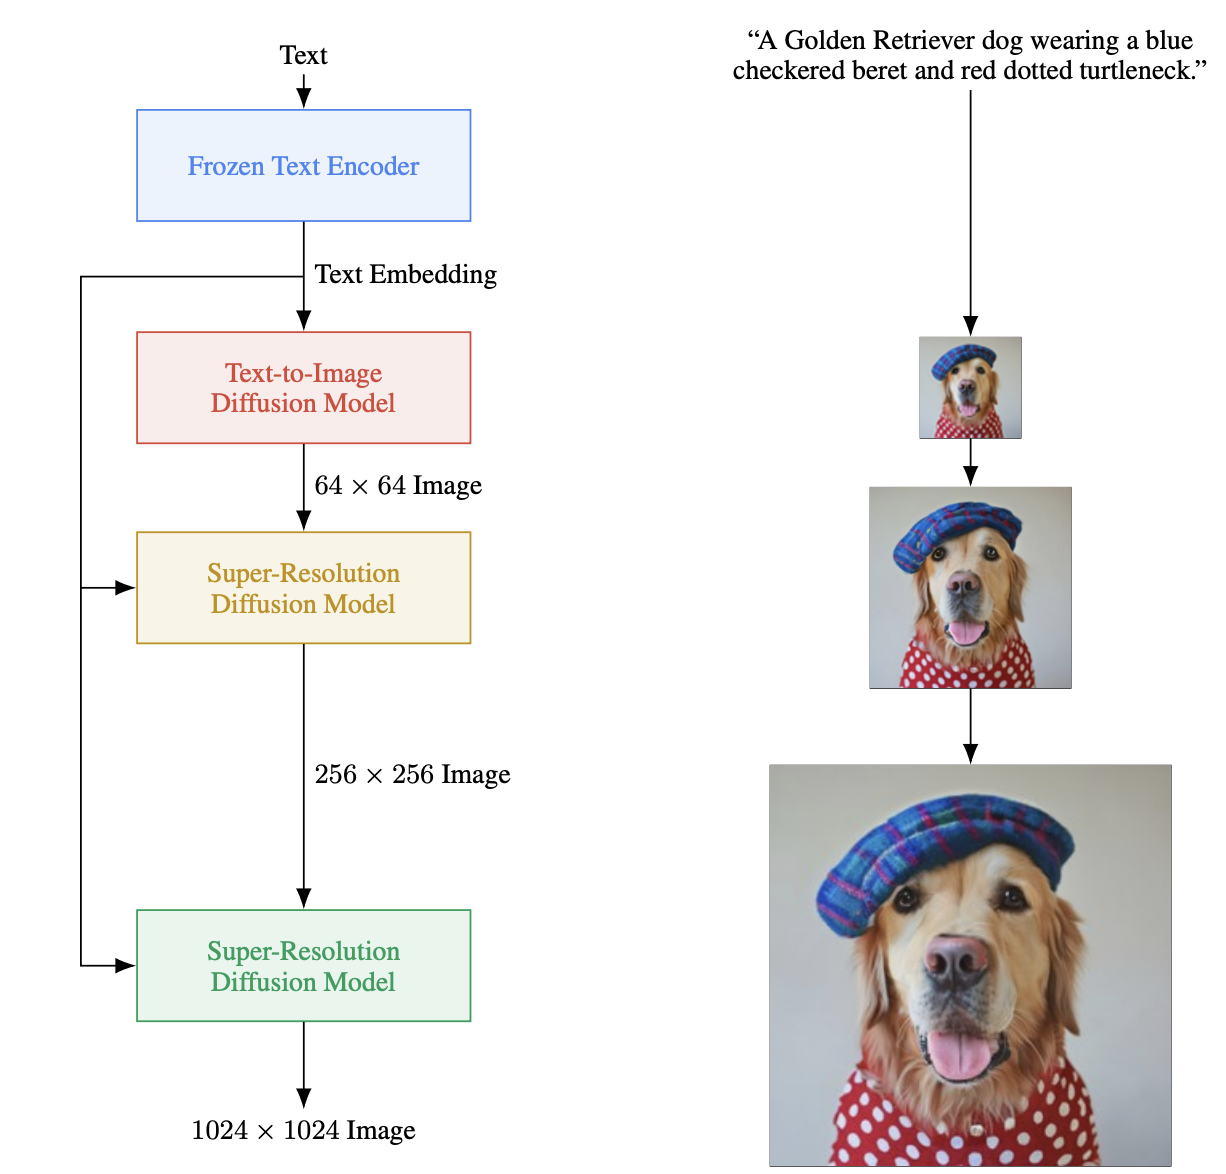
\includegraphics[width=0.5\textwidth]{images/imagen/architecture.png}
    \caption{Overview of Imagen architecture.}
    \label{fig:imagen_architecture}
\end{figure}

Imagen depends critically on classifier-free guidance \ref{subsec:classifier_free_diffusion_guidance} for effective text conditioning.






